\documentclass[a4paper, 12pt, openany]{report}

\usepackage{amssymb, amsthm, amsfonts, amsmath, mathtools, mathrsfs}
\usepackage{newtxmath, newtxtext}
% \usepackage{fourier}
\usepackage[a4paper]{geometry}
\usepackage[english]{babel}
\usepackage{verbatim}
\usepackage{tikz}
\usepackage{frontespizio}
\usepackage[T1]{fontenc}
\usepackage[utf8]{inputenc}
\usepackage{hyperref}
\usepackage{subcaption}
\usepackage{float}
\usepackage{multicol}
\usepackage{listings}
\usepackage{xcolor} % per i colori

\lstset{
    language=Matlab,          % puoi cambiare in Python, C++, ecc.
    basicstyle=\ttfamily\footnotesize,
    keywordstyle=\color{blue},
    commentstyle=\color{green!50!black},
    stringstyle=\color{red},
    numbers=none,
    numberstyle=\tiny\color{gray},
    stepnumber=1,
    numbersep=2pt,
    showstringspaces=false,
    breaklines=true,
    frame=none
}

\hypersetup{
  colorlinks=false,
  pdfborder={0 0 0} % forza border a zero
}

\DeclareMathSizes{10}{10}{7}{5}
% \numberwithin{equation}{section}

\newtheoremstyle{myplain}% Custom style for theorems
    {1ex}% Space above
    {1ex}% Space below
    {\itshape}% Body font
    {}% Indent amount
    {\bfseries}% Theorem head font
    {.}% Punctuation after theorem head
    {0.5em}% Space after theorem head
    {}% Theorem head spec

\newtheoremstyle{mydefinition}% Custom style for definitions and similar environments
    {1ex}% Space above
    {1ex}% Space below
    {\normalfont}% Body font
    {}% Indent amount
    {\bfseries}% Theorem head font
    {.}% Punctuation after theorem head
    {0.5em}% Space after theorem head
    {}% Theorem head spec

\theoremstyle{myplain}
\newtheorem{theorem}{Theorem}[section]
\newtheorem{proposition}[theorem]{Proposition}
\newtheorem{lemma}[theorem]{Lemma}
\newtheorem{corollary}[theorem]{Corollary}

\theoremstyle{mydefinition}
\newtheorem{definition}[theorem]{Definition}
\newtheorem{example}[theorem]{Example}
\newtheorem{remark}[theorem]{Remark}

\newcommand{\R}{\mathbb{R}}
\newcommand{\C}{\mathbb{C}}
\newcommand{\bigO}{\mathcal{O}}
\newcommand{\kron}{\otimes}
\newcommand{\abs}[1]{\left| #1 \right|}
\newcommand{\ii}{\mathrm{i}}
\newcommand{\dd}{\mathrm{d}}
\newcommand{\ddiv}{\mathbf{\nabla} \cdot}
\newcommand{\xx}{\mathbf{x}}
\newcommand{\hh}{\mathbf{h}}
\newcommand{\rr}{\mathbf{r}}
\newcommand{\uu}{\mathbf{u}}
\newcommand{\nb}{\mathbf{\nabla}}
\newcommand{\pdv}[2]{\frac{\partial #1}{\partial #2}}
\newcommand{\pdvn}[3]{\frac{\partial^{#3} #1}{\partial #2^{#3}}}
\newcommand{\lap}{\laplace}
% \newcommand{\lap}{\mathbf{\Delta}}

\renewcommand{\thetheorem}{\thechapter.\arabic{theorem}}
\renewcommand{\qedsymbol}{$\blacksquare$}

\begin{document}

\begin{Preambolo*}
    \usepackage{newtxtext}
\end{Preambolo*}

\begin{frontespizio}

    \Universita{Verona}
    \Facolta{Scienze e Ingegneria}
    \Corso[laurea triennale]{Matematica Applicata}
    \Logo{img/logo_univr_png}
    \Annoaccademico{2024--2025}
    \Titoletto{Tesi di laurea triennale}
    \Titolo{Numerical Simulations of Vortex Dynamics in Quantum Fluids}
    \Sottotitolo{}
    \Candidato[VR489417]{Alessio Zanella}
    \Relatore{Marco Caliari}

\end{frontespizio}

\tableofcontents

% introduction
\chapter{Introduction}

\section{Introduction to superfluidity}

The equations of classical fluid dynamics, such as the Navier-Stokes equations, have been known for more than a century. However, the complete understanding of their solutions in a turbulent regime remains one of the most important unsolved problems in classical physics.

Strangely, in the context of quantum mechanics, there exists quantum entities called bosons, as they respond to Bose-Einstein statistics, unlike Fermions, which follows the Fermi-Dirac statistics. At temperatures approaching absolute zero,these exhibit peculiar behaviors, in particular they can occupy the same quantum state, which fermions cannot, due to the Pauli exclusion principle. As a result, when a large number of bosons are cooled, a condensate is formed. This collective behavior gives rise to remarkable phenomena, such as superfluidity.

In this condensed state, the behavior of the superfluid is described by a single wave function, which carries both density and motion information. The dynamical evolution of this function is given by the Schrödinger equation, which, in our case, is called the Gross-Pitaevskii equation (GPE), a nonlinear form of the above equation.

Of course, since it is still a fluid, vorticity phenomena can occur, with the latter evolving by moving and recombining, thus establishing the relationship with classical fluid dynamics. In this framework, numerical simulations play a fundamental role, as the GPE is difficult to solve analytically, especially in the presence of vortices and complex phenomena such as the evolution and recombination of the latter. 

The aim of this thesis is to study in detail an efficient numerical method for the resolution of GPE in the presence of vortices, both from the point of view of numerical analysis and by performing some experiments. 

\newpage

\section{The mathematical context}

In this section we introduce the mathematical model for a superfluid and seek an analytical approximation for the density $\rho$.

We define a \emph{two-dimensional vortex} as a vortex filament embedded in three-dimensional space that possesses cylindrical symmetry. Assuming its axis lies along the $x_3$-direction, the configuration depends only on the coordinates in the orthogonal plane, so that variations are observed exclusively in the $(x_1,x_2)$-plane.

The governing equation for a weakly interacting Bose-Einstein condendate is the \emph{Gross-Pitaevskii equation} (GPE for short)

\begin{equation*}
    \ii \hbar \pdv{\psi}{t} = -\frac{\hbar^2}{2m}\lap\psi + V_0\abs{\psi}^2 \psi - E_0 \psi
\end{equation*}

where $\psi = \psi(\rr, t)$ is the complex macroscopic wavefunction for a condensate of $N$ bosons of mass $m$ at position $\rr$ and time $t$. The constant $\hbar$ is the reduced Planck's constant, $V_0$ is the strength of the repulsive interactions between bosons, and $E_0$ is the chemical potential of the system (the energy required to add a boson to the condensate).

The adimensional form of the GPE, which derivation can be found in \cite{CZ12}, is

\begin{equation}
    \pdv{\psi}{t} = \frac\ii2\lap\psi + \frac\ii2 (1 - \abs{\psi}^2)\psi
    \label{eq:gpe}
\end{equation}

Let us introduce the Madelung transformation, writing the wavefunction in polar form

\begin{equation}
    \psi(\rr, t) = \rho^{1/2}\exp(\ii S)
    \label{eq:madelung}
\end{equation}

where $\rho = \rho(\rr, t) = \abs{\psi(\rr, t)}^2$ is the density and $S = S(\rr, t)$ is the phase of $\psi$. The vector field $\uu = \nb S$ can be interpreted as the superfluid velocity field.

\medskip

Substituting \eqref{eq:madelung} into \eqref{eq:gpe} and separating real and imaginary parts, we obtain the following system of equations, written in Einstein notation

\begin{align*}
    &\pdv{\rho}{t} + \pdv{\rho u_j}{x_j} = 0 \\
    &\rho \left(\pdv{u_i}{t} + u_j \pdv{u_i}{x_j}\right) = -\pdv{p}{x_i} + \pdv{\tau_{ij}}{x_j}, \quad i = 1,2,3
\end{align*}

where 

\[
    p = \frac{\rho^2}{4} \quad \text{and} \quad \tau_{ij} = \frac14 \rho \pdvn{\log \rho}{x_i x_j}{2}
\]

are the pressure and the quantum stress tensor, respectively. 

These equations resemble the classical Navier-Stokes equations for a barothopic, inviscid fluid, where the volume forces are conservative (in our case they are constantly zero). The main difference is in the stress term, since a quantum fluid is inviscid, and the stress is not proportional to the strain rate tensor, but rather to the second derivatives of the logarithm of the density.

\subsection{Approximation of steady-state vortex}

In a two-dimensional domain we set $\psi(x,y) = \rho\left(\sqrt{x^2 + y^2}\right)\exp\left(\ii \theta(x,y)\right)$, where $\rho(r)$ is a function to be determined. By imposing the non dependence by the time (steady state solution), we obtain that $\rho$ has to satisfy

\begin{equation}
    \rho'' + \frac{\rho'}{r} + \frac{(\rho')^2}{2\rho} - \frac{2\rho}{r^2} + 2(1 - \rho)\rho = 0
    \label{eq:density}
\end{equation}





% numerical methods
\chapter{Numerical Methods}

\section{Space discretization}

In this section we describe the spatial discretization methods used to simulate the GPE.

\subsection{Finite differences on uniform grid}

Let us discretize the interval $[-L, L]$ with $m$ equispaced points, so that 
\[
    x_1 = -L, \quad x_m = L, \quad x_j = -L + (j-1)h, \quad 1 \leq j \leq m,
\]

where the mesh size is given by $h = \tfrac{2L}{m-1}$.  
Following \cite{dispenseCaliari}, the second derivative along one spatial direction is approximated by the standard finite-difference matrix

\[
    D_{2}^x = \frac{1}{h^2}
    \begin{bmatrix}
        -2 & 2  & 0  & 0  & \cdots & 0  & 0 \\
        1 & -2 & 1  & 0  & \cdots & 0  & 0 \\
        0 &  1 & -2 & 1  & \cdots & 0  & 0 \\
        0 &  0 &  1 & -2 & \ddots & 0  & 0 \\
        \vdots & \vdots & \ddots & \ddots & \ddots & \vdots & \vdots \\
        0 &  0 &  0 &  \dots & 1 & -2 & 1 \\
        0 &  0 &  0 &  0 & \cdots &  2 & -2
    \end{bmatrix}
\]

This corresponds to the usual second-order central difference scheme with Neumann boundary conditions. 

\subsection{Finite differences on non uniform grid}
\label{sb:nufg}

Although the above numerical scheme is simple and easy to implement, in our case it is not the most suitable one, since, as we will see in the next chapter, it requires a very large number of points to obtain physically reliable results, especially when integrating over long time intervals.  

Given that the vortex density exhibits stronger variations near its core, while remaining almost constant towards the boundary of the domain, it would be preferable to employ a grid that clusters points around the vortex center(s). 
In this way, higher resolution is achieved in the regions where sharp variations occur.

Consider the interval $[a,b]$ and let $\xx = [x_1, \dots, x_m]^T$, with 

\[
    x_1 = a, \quad x_m = b, \quad x_j = x_{j-1} + h_j,
\]

where the grid spacings satisfy $h_j = (1 + \delta) h_{j-1}$ for some fixed parameter $\delta$.  
This leads to the recurrence

\begin{align*}
    h_j &= (1 + \delta) h_{j-1} \\
        &= (1 + \delta)^2 h_{j-2} \\
        &\;\;\vdots \\
        &= (1 + \delta)^{j-1} h_1.
\end{align*}

The constraint is that the sum of all step sizes must cover the entire interval length, which gives
\[
    \sum_{j=1}^{m-1} h_j
    = h_1 \sum_{j=1}^{m-1} (1+\delta)^{j-1} 
    = b-a.
\]

There are three natural ways to proceed, each consisting of fixing two among the parameters $\delta$, $m$, and $h_1$, and then computing the remaining one.  
In what follows, we present two cases: computing $m$ and computing $h_1$.

First of all, we observe that the sum is a geometric series with ratio $1+\delta$, whose closed-form expression is known analytically:  
\[
    \sum_{j=1}^{m-1} (1+\delta)^{j-1} = \frac{(1+\delta)^{m-1} - 1}{\delta}.
\]

To compute $m$ we proceed as follows:

\begin{align*}
    h_1 \frac{(1+\delta)^{m-1} - 1}{\delta} = b-a 
    &\iff (1+\delta)^{m-1} = \frac{\delta(b-a)}{h_1} + 1 \\
    &\iff (m-1)\log(1+\delta) = \log\!\left(\frac{\delta(b-a)}{h_1} + 1\right) \\
    &\iff m = \left\lceil \frac{\log\!\left(\tfrac{\delta(b-a)}{h_1} + 1\right)}{\log(1+\delta)} + 1 \right\rceil.
\end{align*}

Since $m$ must be an integer, we take the ceiling in the final expression.

The expression for $h_1$, after some trivial algebra, is

\[ h_1 = \frac{\delta(b - a)}{1 - (1 + \delta)^{m - 1}} \]

To construct the one-dimensional discretization, it is important to note that, in the case of non-uniform finite differences, the local error can be shown to be proportional to $\bigO(h_j^2)$ provided that the difference between $h_j$ and $h_{j-1}$ is of order $\bigO(\max\{h_j^2, h_{j-1}^2\})$, therefore, care must be taken in constructing the grid using the above formula, so as to keep the difference between two consecutive steps as smooth as possible. Otherwise, the error would not even be proportional to $h_j$, which in the worst case would lead to an inconsistent scheme and consequently to significant errors in the time integration.

With this in mind, we can construct the discretization along one direction by applying the procedure described above to the interval $[0, x_c]$, where $x_c$ denotes the center of the vortex, clustering the points towards $x_c$.  
We then extend the grid from $x_c$ to the boundary of the domain, using the same values of $h$ and $\delta$, so that the spacing over the interval $[0, 2x_c]$ remains consistent with the previous construction.  
The grid can be further extended up to the domain boundary within a small tolerance, since this procedure does not necessarily guarantee that the endpoints are reached exactly.  
However, this is not problematic, as small discrepancies at the domain boundaries do not significantly affect the evolution of the dynamics, being far from the regions of interest.

Once we have the step vector $\hh$ constructed, we can discretize the second derivative along one direction using the tridiagonal matrix

\[
    D_2^x =
    \begin{bmatrix}
        -\frac{2}{h_1^2} & \frac{2}{h_1^2} & 0 & \dots & 0 \\
        \frac{2}{h_2(h_1+h_2)} & -\frac{2}{h_1 h_2} & \frac{2}{h_1(h_1+h_2)} & \dots & 0 \\
        0 & \frac{2}{h_3(h_2+h_3)} & -\frac{2}{h_2 h_3} & \ddots & 0 \\
        \vdots & \ddots & \ddots & \ddots & \frac{2}{h_{m-1}(h_{m-2}+h_{m-1})} \\
        0 & \dots & 0 & \frac{2}{h_{m-1}^2} & -\frac{2}{h_{m-1}^2}
    \end{bmatrix}
\]

\subsection{Laplacian discretization}

Now, in both cases (uniforn or not), the Laplacian operator in two dimension is approximated by 

\begin{equation}
    \lap \approx I^y \kron D_2^X + D_2^Y \kron I^x
    \label{eq:lapprox}
\end{equation}

where $\kron$ denotes the Kronecker product (see \ref{ch:krondef} for further details), and $I^*$ denotes the identity matrix of the dimension equal to the number of points in each direction.

\section{Time integration}

\subsection{Strang splitting method}

Consider the Cauhcy problem

\begin{equation}
    \begin{cases}
        \pdv{u}{t} = (A + B) u \\
        u(0) = u_0
    \end{cases}
    \label{eq:cauchy}
\end{equation}

\begin{proposition}
    If $A$ and $B$ commute, then $\exp(A+B) = \exp(A)\exp(B)$
\end{proposition}

\begin{proof}
    
    \begin{align*}
        \exp(A + B) &= \sum_{n = 0}^\infty \frac{(A + B)^n}{n!} \\
                    &= \sum_{n = 0}^\infty \sum_{k = 0}^n \binom{n}{k} \frac{A^k B^{n-k}}{n!} \\
                    &= \sum_{n = 0}^\infty \sum_{k = 0}^n \frac{A^k}{k!} \frac{B^{n - k}}{(n - k)!}  \quad \ell = n - k \\
                    &= \sum_{k = 0}^\infty \frac{A^k}{k!} \sum_{\ell = 0}^\infty \frac{B^\ell}{\ell!} \\
                    &= \exp(A)\exp(B)
    \end{align*}

\end{proof}

The analytical solution for \ref{eq:cauchy} is

\[ u(t) = e^{(A + B)t} u_0 \]

So, for the previous proposition, if $A$ and $B$ commute, then $u(t) = e^{tA}e^{tB}u_0 \implies u(t + \tau) = e^{\tau A}e^{\tau B}u(t)$.

This is equivalent to solve separately two initial value problems:

\[
    \begin{cases}
        \pdv{u}{t} = A u \\
        u(0) = u_0
    \end{cases}
    \label{eq:subproblemA}
\]

and

\[
    \begin{cases}
        \pdv{u}{t} = B u \\
        u(0) = u_0
    \end{cases} 
\]

This gives rise to a numerical scheme:

\[
    \begin{aligned}
        \bar{u}_{n+1} &= \exp(\tau A)u_n \\
        u_{n+1} &= \exp(\tau B)\bar{u}_{n+1}
    \end{aligned}
\]

This approach is known as \emph{Lie splitting}. It is exact when the operators $A$ and $B$ commute, otherwise it achieves first-order accuracy with respect to the time step $\tau$.

Other methods can be constructed by considering alternative ways of splitting the operators. One widely used approach is the \emph{Strang time splitting}, which improves the accuracy by symmetrically composing the substeps. Specifically, it provides the numerical scheme

\begin{equation}
    \begin{aligned}
        \bar{u}_{n+1} &= \exp\left(\frac\tau2 A\right)u_n \\
        \tilde{u}_{n+1} &= \exp(\tau B)\bar{u}_{n+1} \\
        u_{n+1} &= \exp\left(\frac\tau2 A\right)\tilde{u}_{n+1}
    \end{aligned}
\end{equation}

where $u_n \approx u(t_n)$.

\begin{proposition}[Error of Strang splitting]
    The Strang time-splitting method is \emph{exact} if the operators $A$ and $B$ commute, and it is of order $2$ with respect to the time step $\tau$ otherwise.
\end{proposition}

\begin{remark}
    In the special case where $A$ and $B$ commute, the Strang splitting becomes exact. Indeed, we have
    \[
        e^{(A+B)\tau} = e^{\tau A} e^{\tau B} 
        = e^{\frac{\tau}{2} A} e^{\frac{\tau}{2} A} e^{\tau B} 
        = e^{\frac{\tau}{2} A} e^{\tau B} e^{\frac{\tau}{2} A},
    \]
    which coincides with the splitting formulation.
\end{remark}

\begin{proof}[Order 2]
    Let us now consider the general case where $A$ and $B$ do not commute. 
    The exact solution after one time step is given by
    \[
        u(t+\tau) = e^{(A+B)\tau} u(t),
    \]
    whereas the Strang approximation reads
    \[
        u(t+\tau) \approx e^{\frac{\tau}{2}A} e^{\tau B} e^{\frac{\tau}{2}A} u(t).
    \]

    The difference between the two is entirely contained in the discrepancy between the operators
    \[
        e^{(A+B)\tau} \quad \text{and} \quad e^{\frac{\tau}{2}A} e^{\tau B} e^{\frac{\tau}{2}A}.
    \]

    To quantify this, we expand the Strang operator in a Taylor series:
    \[
        \left( I + \tfrac{\tau}{2}A + \tfrac{\tau^2}{8}A^2 + \bigO(\tau^3) \right)
        \left( I + \tau B + \tfrac{\tau^2}{2}B^2 + \bigO(\tau^3) \right)
        \left( I + \tfrac{\tau}{2}A + \tfrac{\tau^2}{8}A^2 + \bigO(\tau^3) \right).
    \]

    Multiplying and collecting terms up to order $\tau^2$, we obtain
    \[
        I + \tau(A+B) + \tfrac{\tau^2}{2}(A+B)^2 + \bigO(\tau^3).
    \]

    On the other hand, the Taylor expansion of the exact propagator is
    \[
        e^{(A+B)\tau} = I + \tau(A+B) + \tfrac{\tau^2}{2}(A+B)^2 + \tfrac{\tau^3}{3}(A+B)^3 + \bigO(\tau^4).
    \]

    Subtracting the two expressions shows that the leading term of the local error is of order $\tau^3$. Hence, the method is (at least) second-order accurate.

    To prove that it is \emph{exactly} 2, we need to expand up to the third order and subtract. After some computation, one finds that the local error is 

    \[
        \tau^3 \left( \frac{1}{12}\left[B, \left[B, A\right]\right] - \frac{1}{24} \left[A, \left[A,B\right]\right]\right) + \bigO(\tau^4) = \bigO(\tau^3)
    \]

    Since the cubic terms do not cancel, the method has a local error proportional to $\tau^3$, and is therefore of order 2.
\end{proof}

\begin{figure}
    \centering
    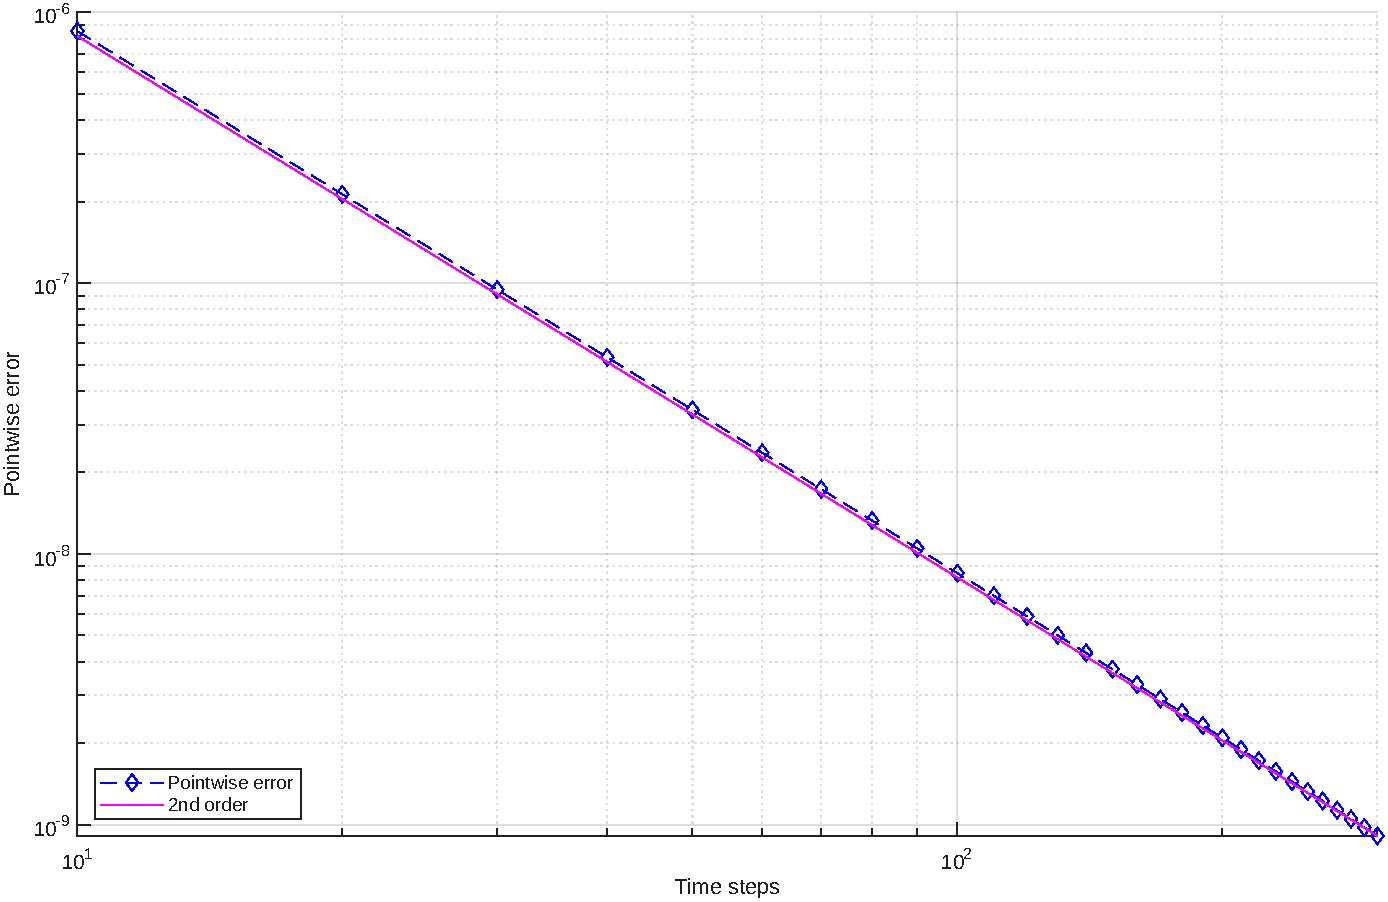
\includegraphics[width=0.8\textwidth]{img/time_conv.pdf}
    \caption{Convergence order}
\end{figure}


\subsection{Method applied to GPE}

In the case of GPE, we have $A = \frac\ii2 \lap$ and $B = \frac\ii2 \left(1 - \abs{u}^2\right)$. 

For $B$ we directly approximate the solution. The treatment for the first is more delicate: since in fact the Laplacian operator is approximated by the formula \ref{eq:lapprox}, we need to compute the matrix-vector product 

\[
    \exp\left(\frac\tau2 \left(I^y \kron D_2^x + D_2^y \kron I^x\right)\right)u_n
\]

which, for large matrices, is almost impossible dealing with in computationally reasonable times. Our goal would be avoiding the construction of any Kroneker product; instead we directly compute the action of the latter on the vector $\uu$. First we notice that $I^y \kron D_2^x$ and $D_2^y \kron I^x$ commute, as trivial consequence of the formula \ref{prop:prod}. This implies that 

\[ \exp\left(I^y \kron D_2^x + D_2^y \kron I^x\right) = \exp\left(I^y \kron D_2^x\right)\exp\left(D_2^y \kron I^x\right) \]

Since the exponential function is analytical, using \ref{th:analytic}, we have

\[ \exp\left(I^y \kron D_2^x\right) = I^y \kron \exp\left(D_2^x\right) \]

and the same for the other. Using again the formula \ref{prop:prod}, we obtain 

\[ \exp\left(I^y \kron D_2^x + D_2^y \kron I^x\right)\uu = \left(\exp\left(D_2^y\right) \kron \exp\left(D_2^x\right)\right)\uu \]

This is way better than directly compute the full exponential of Kroneker product, but it still requires the computation of a large full matrix. This can be avoided, since we can take into account the matrix $U = (u_{i,j}) \in \C^{m_x \times m_y}$, with the relation $U_{i,j} = u_{i + m_x(j - 1)}$, also denoted with $\mbox{Vec}(U) = u$. Let now $E_x = \exp\left(\tau D_2^x\right) = e_{i_1, j_1}$ and $E_y = \exp\left(\tau D_2^y\right) = e_{i_2, j_2}$. Thanks to \ref{prop:tensorprod}



% numerical experiments
\chapter{Numerical experiments}

\section{Stationary vortex preservation over long time integration}

The first numerical experiment we consider concerns the preservation of the steady-state solution of \ref{eq:gpe}. Since this solution is stationary, a natural way to assess the quality of our numerical method is to examine how much the approximate solution deviates from the initial one over long integration times.

In all the following experiments, we approximate the density $\rho$ by a 4-th order Padé approximation of the equation \ref{eq:density}

\subsection{Uniform grid}

We now present some results from the performed experiments. The parameters used in the following simulations are: $m_x = m_y = 347$, $n_t = 450$, $t^* = 20$, $L_x = L_y = 30$.

\begin{figure}[H]
    \centering
    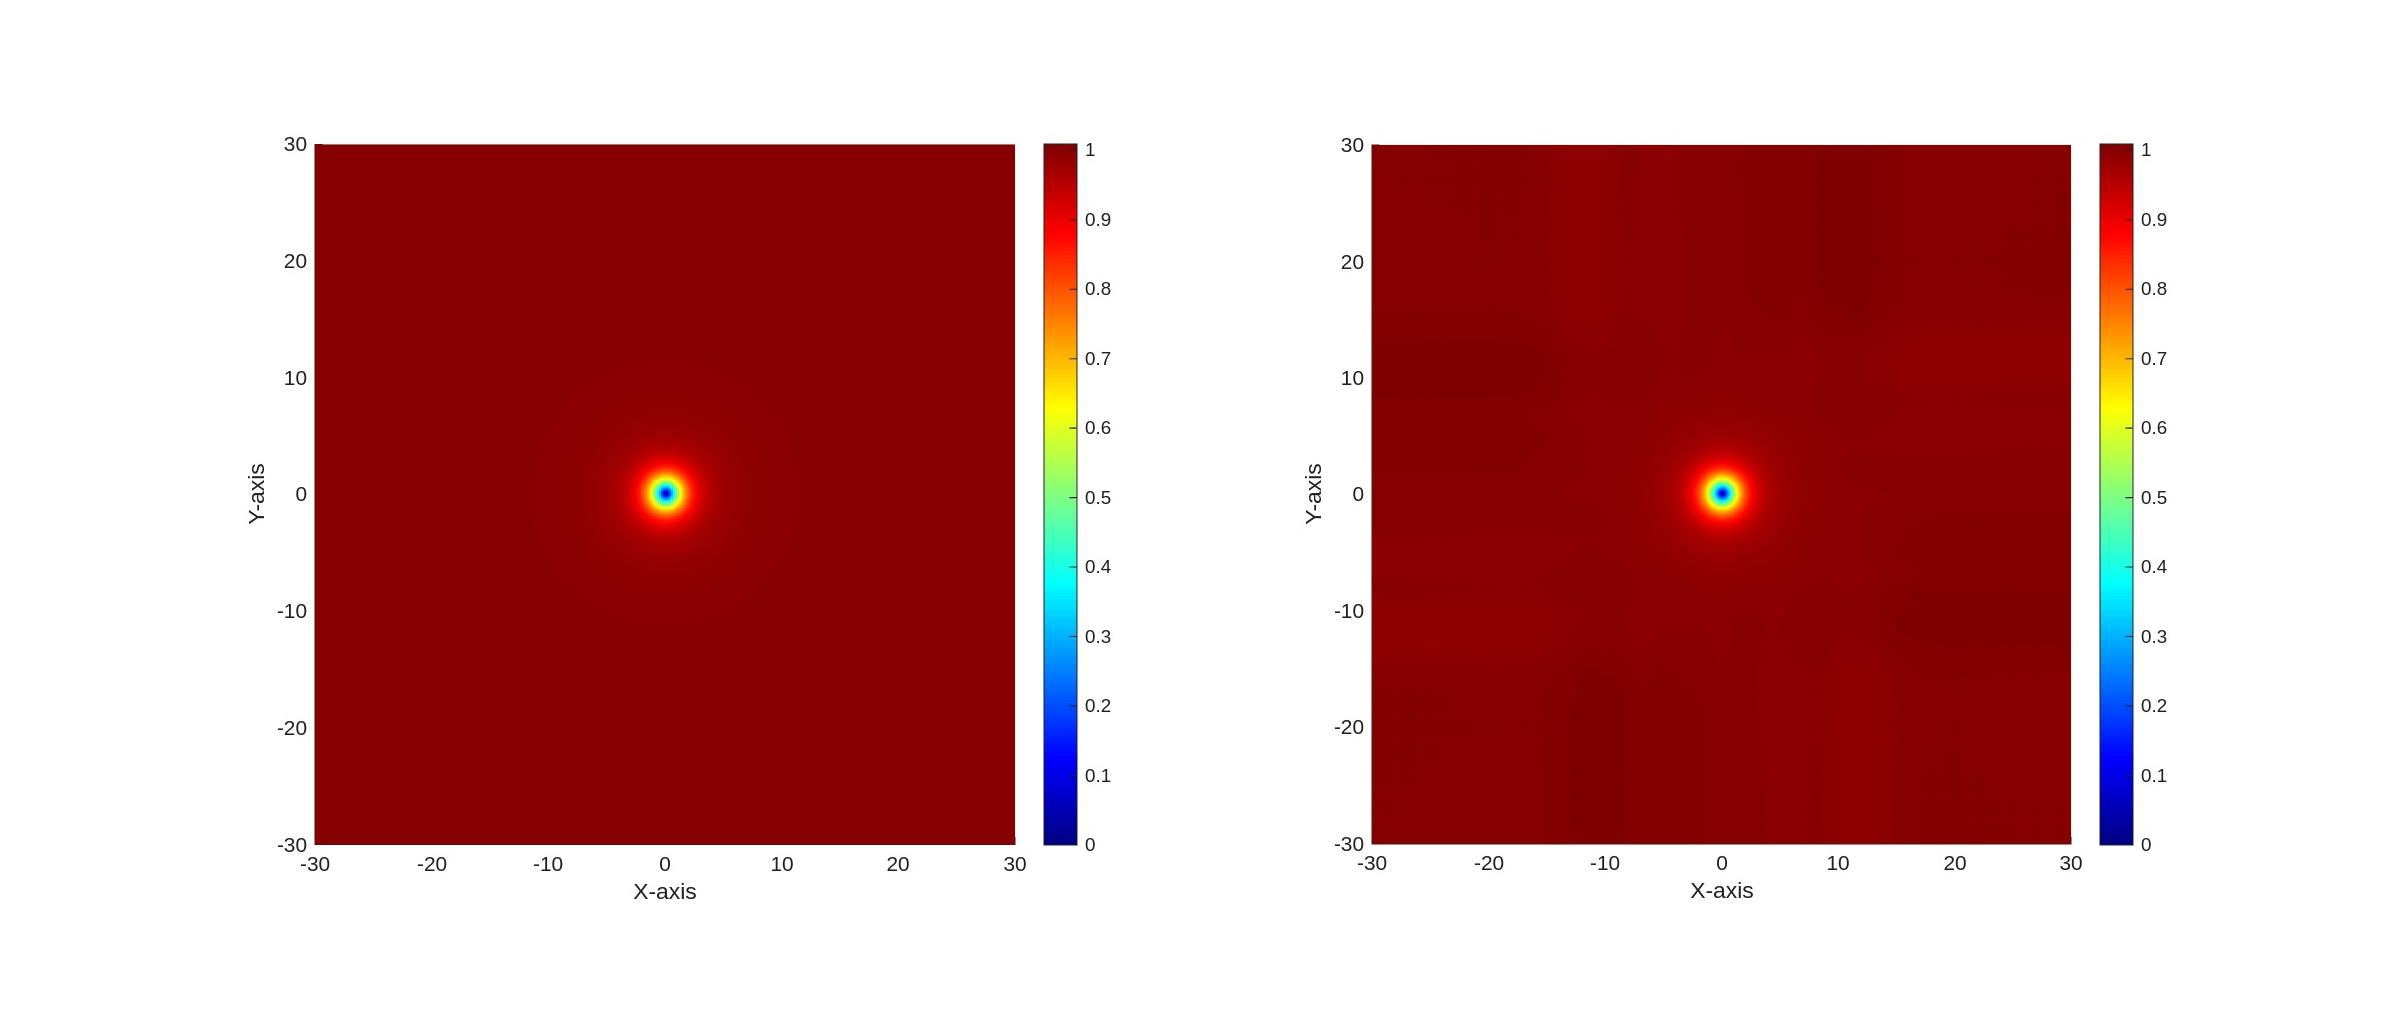
\includegraphics[width=\textwidth]{img/ltufd20t347s30L.pdf}
    \caption{$\abs{\psi_0}$ (left) and $\abs{\psi(20)}$ (right), finite differences on a uniform grid.}
\end{figure}

In this figure, we can observe that the numerical solution integrated up to $t = 20$ shows slight variations in the norm outside the vortex core. To highlight this difference more clearly, we employ an alternative colormap with a steeper gradient for values close to $1$:

\begin{figure}[H]
    \centering
    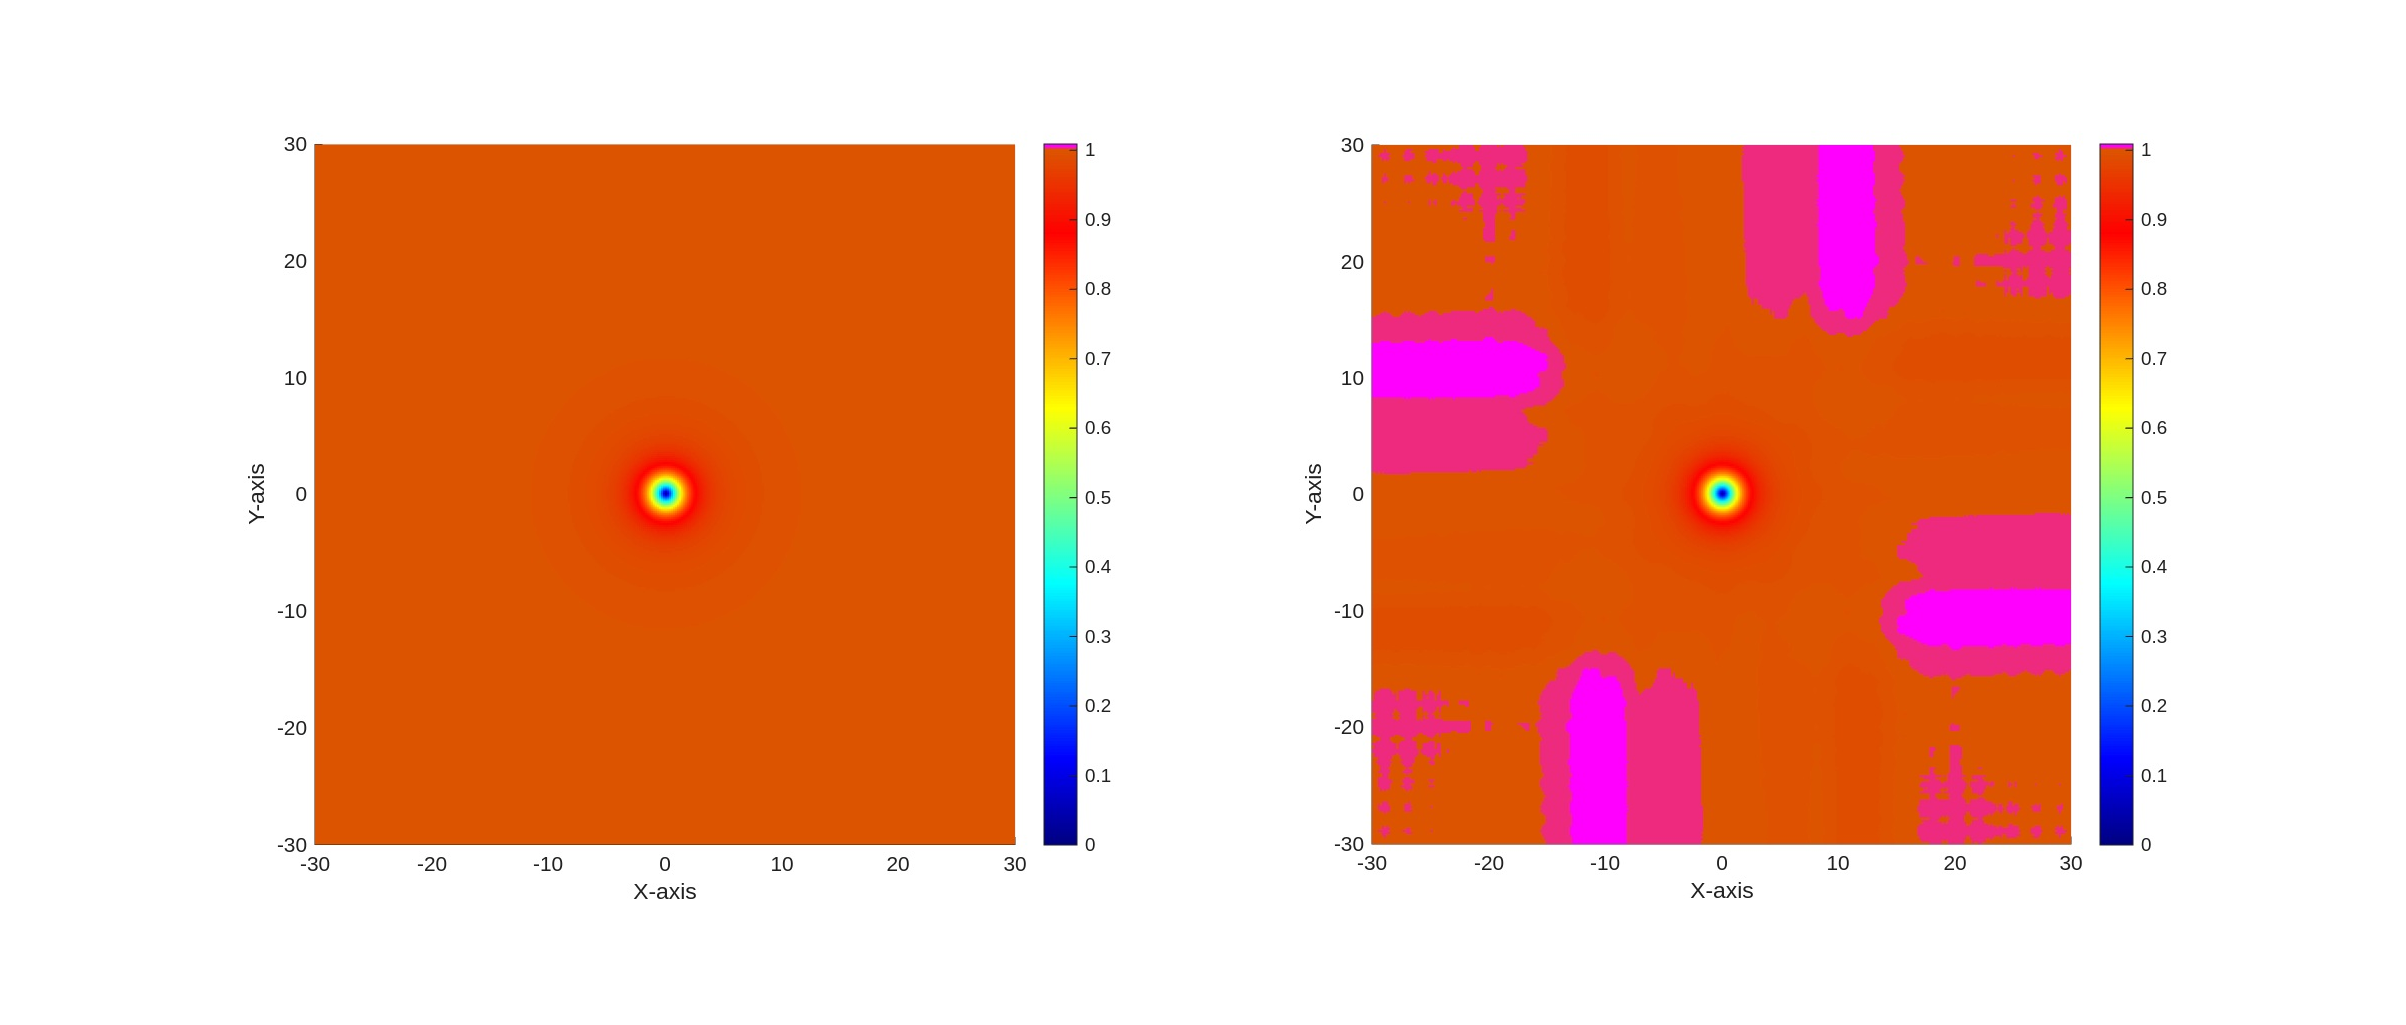
\includegraphics[width=\textwidth]{img/ltufd20t347s30L_color.pdf}
\end{figure}

We observe that the variations in the norm are localized near the limit of the domain, outside the vortex core. To highlight this, Figure~\ref{fig:vortex_center} shows the truncated domain $[-5,5]$, emphasizing the vortex center.

\begin{figure}[H]
    \centering
    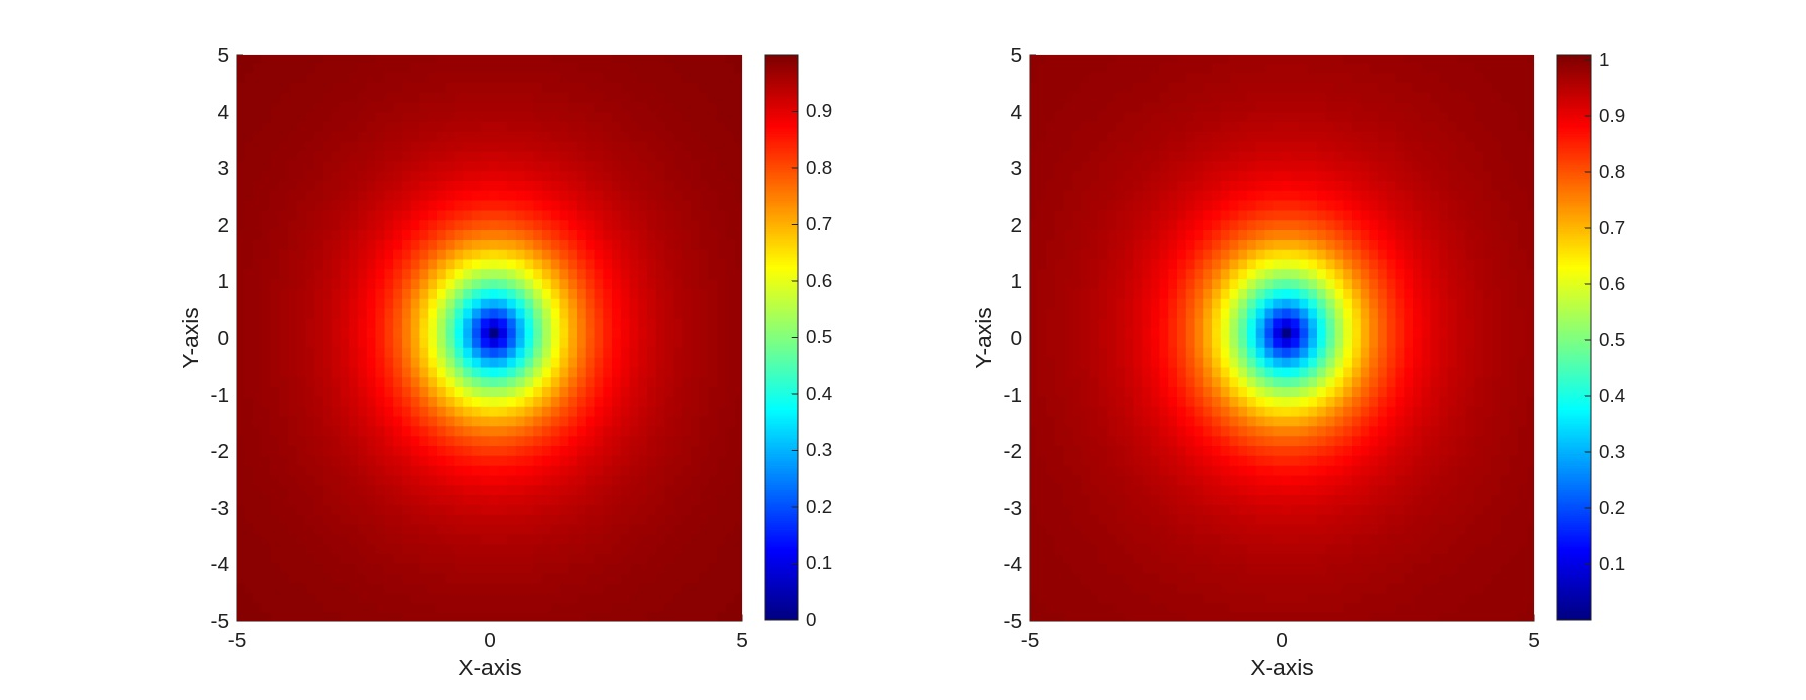
\includegraphics[width=\textwidth]{img/ltufd20t347s30L_5.pdf}
    \caption{Zoomed domain}
    \label{fig:vortex_center}
\end{figure}

From this figure, we can see that no visually appreciable variations occur near the vortex core.

\subsection{Non-uniform grid}

We now consider a non-uniformly spaced grid as described in \ref{sb:nufg}, with $\delta = h_1 = 1/50$. This results in a grid composed of 347 points per direction.

We directly report the comparison between the uniform and non-uniform grids.

\begin{figure}[H]
    \centering
    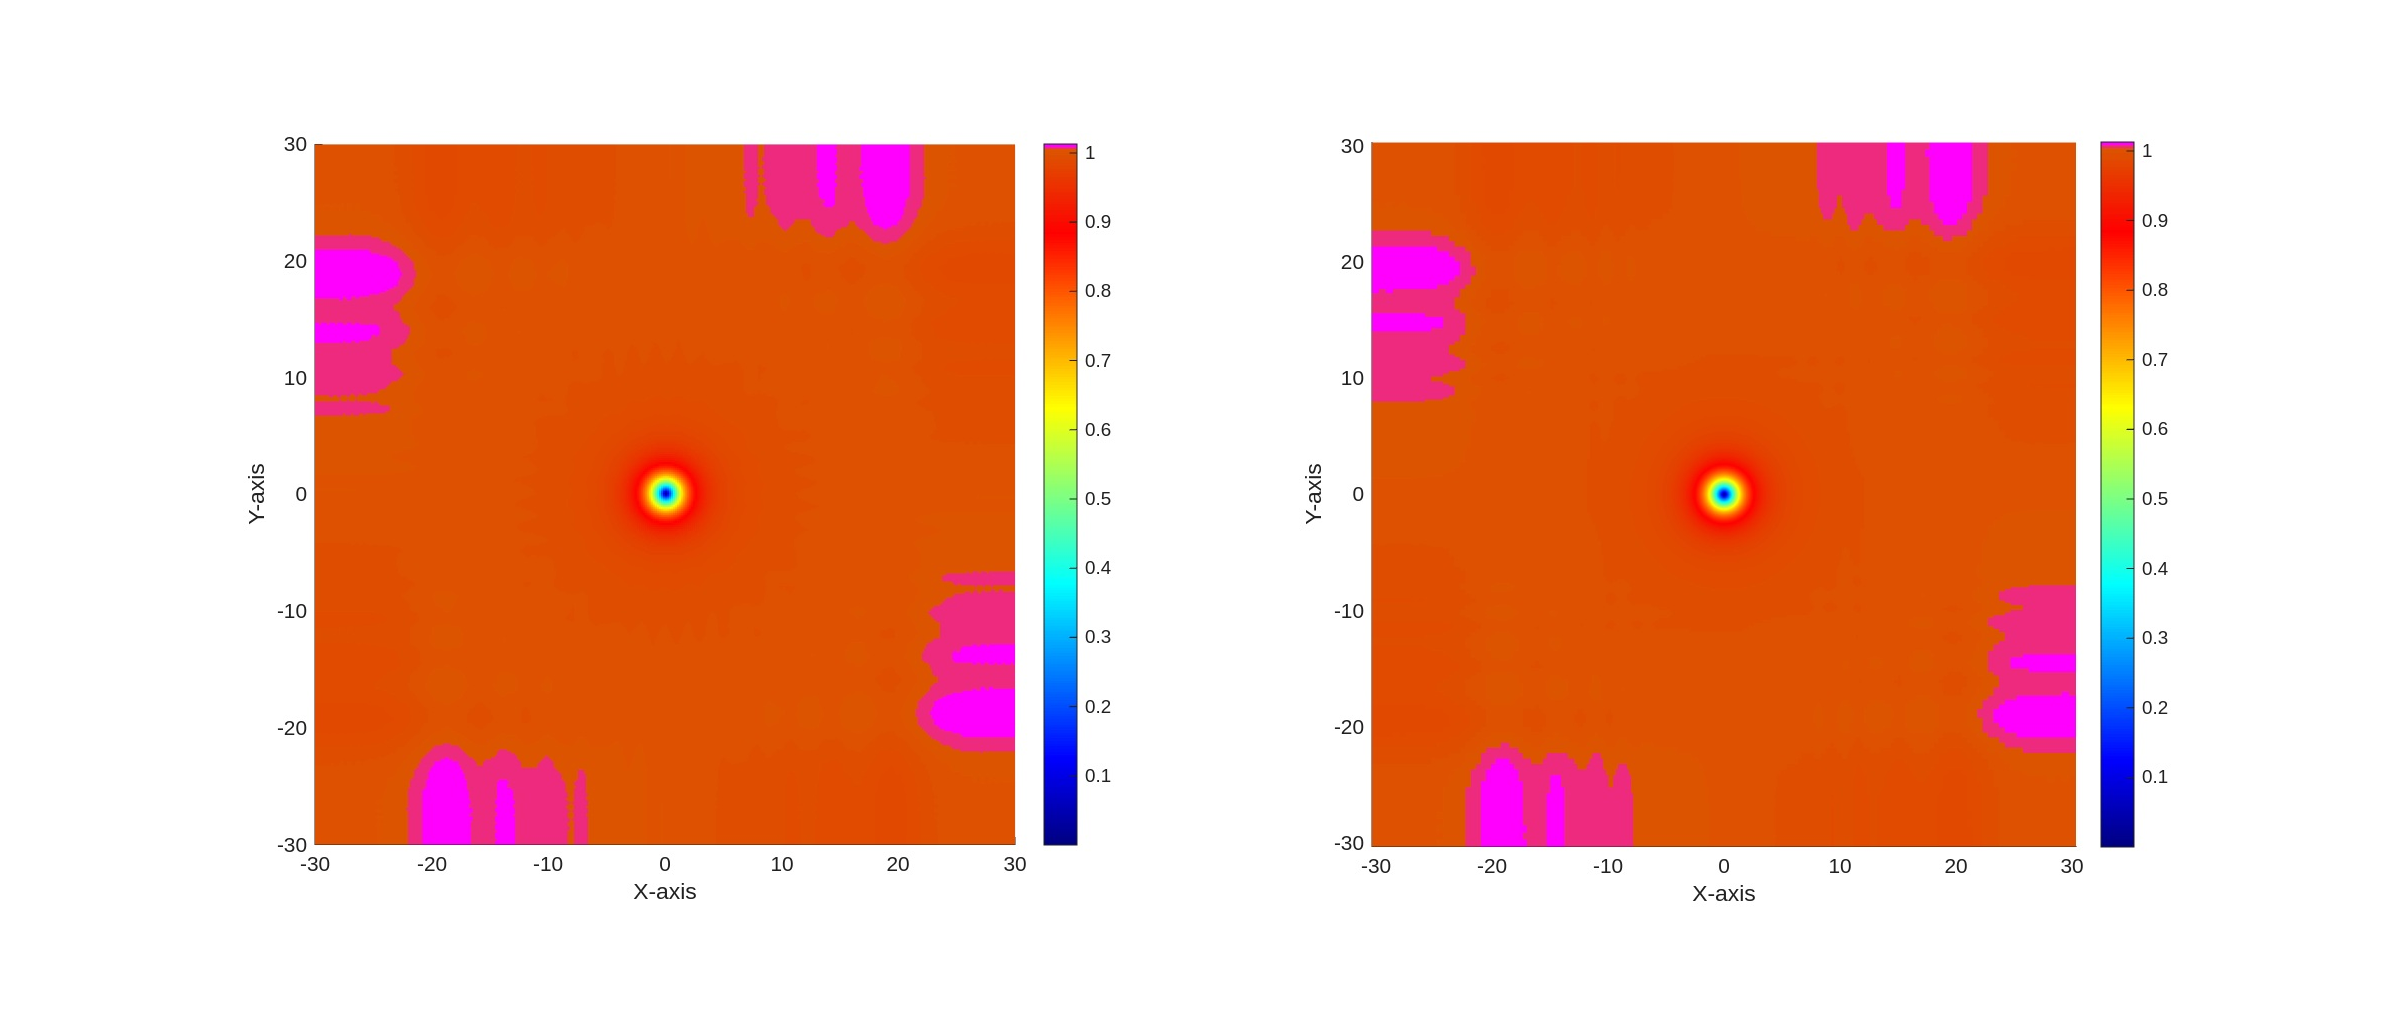
\includegraphics[width=\textwidth]{img/comparison_unfd.pdf}
    \caption{Comparison between uniform (left) and non-uniform (right) grids.}
\end{figure}

We can observe that the solution on the two grids visually differs only near the boundaries of the domain. In the case of the non-uniform grid, the deviation from the uniform grid remains smaller.

\begin{figure}[H]
    \centering
    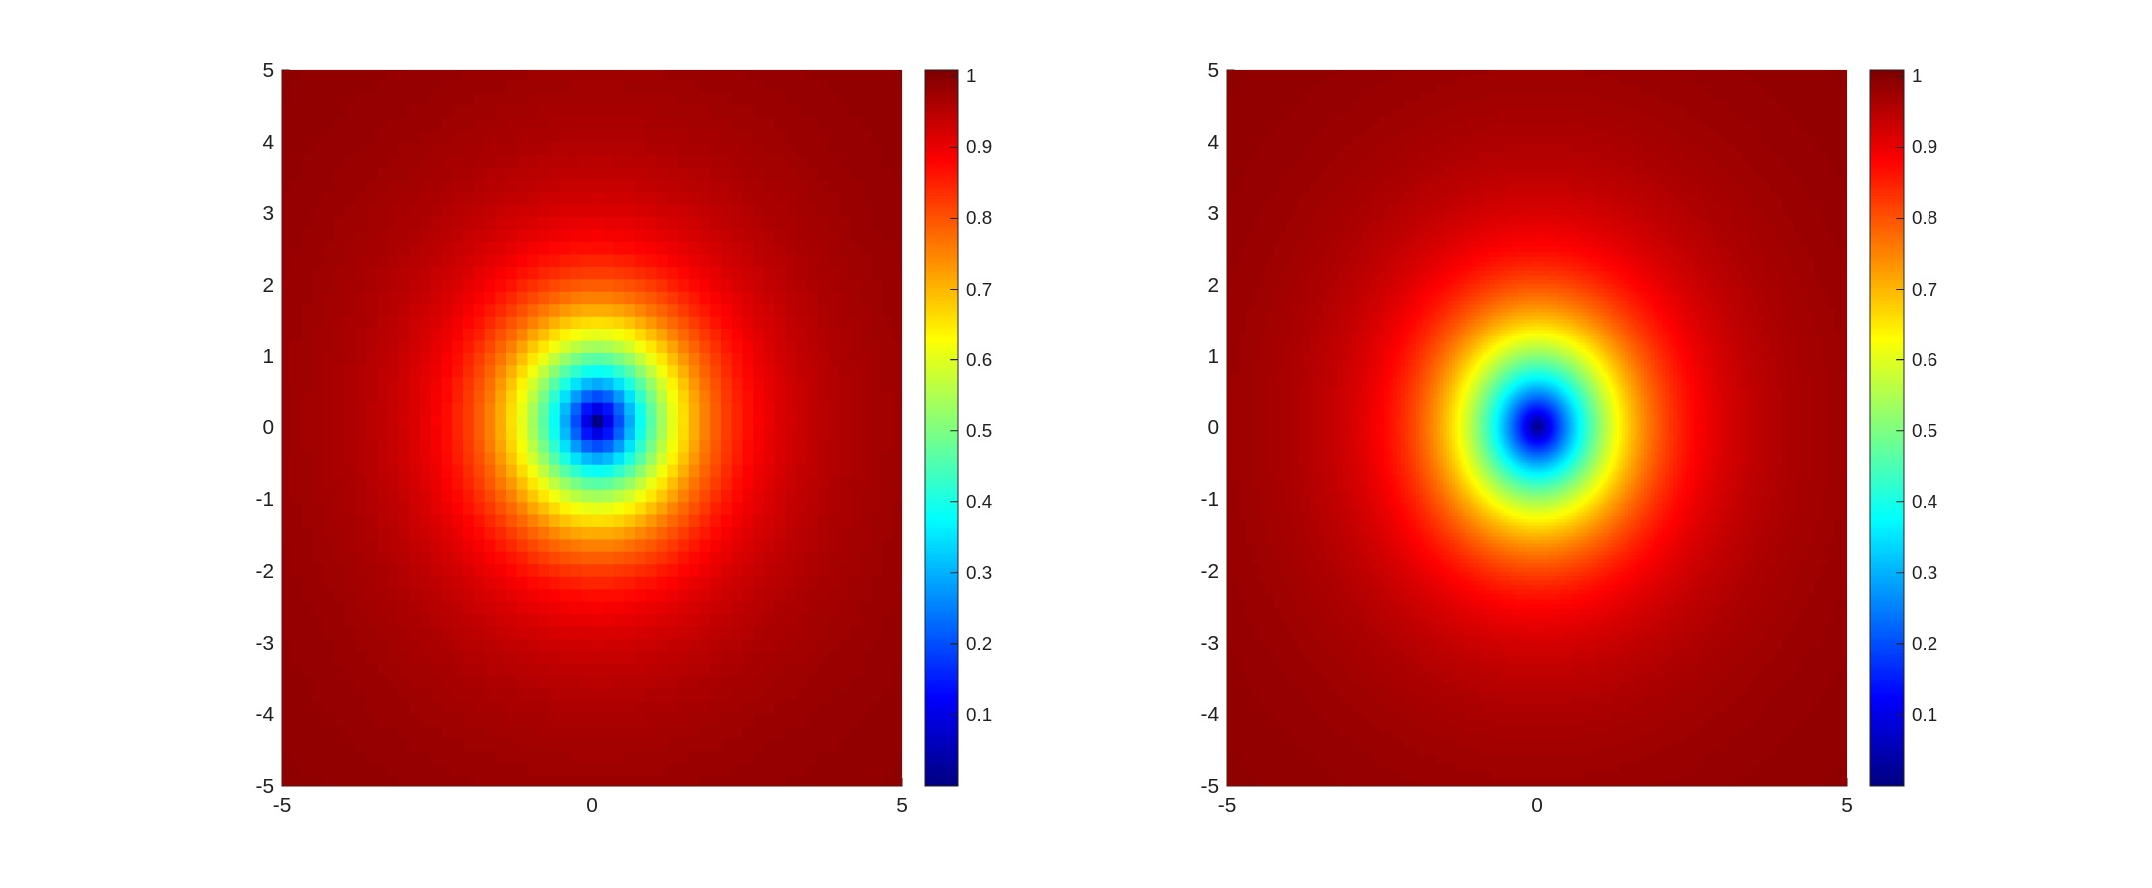
\includegraphics[width=\textwidth]{img/comparison_unfd_5.pdf}
    \caption{Zoom near the center of the domain.}
\end{figure}

Zooming into the center of the domain, no significant differences are observed. However, the refinement of the grid towards the origin in the non-uniform construction is clearly visible.

\section{Simulations of two straight vortices}

In this section, we simulate the dynamics of two interacting straight vortices. We perform experiments by imposing both concordant and opposite initial phases, and compare the different spatial discretization methods introduced so far.

\subsection{Simulation of ''marching'' vortices}

We now proceed to perform a set of simulations involving two straight vortices, centered respectively at $(x_{c_1}, y_{c_1})$ and $(x_{c_2}, y_{c_2})$. In this case we impose counter-rotating phases, meaning that, given the initial condition 
\[
    \psi_0 = \sqrt{\rho_1 \rho_2}\exp\bigl(\ii (S_1 + S_2)\bigr),
\] 
we have $\rho_1 = \rho(x - x_{c_1}, y - y_{c_1})$ and $S_1 = \mathrm{atan2}(y - y_{c_1}, x - x_{c_1})$, while $\rho_2 = \rho(x - x_{c_2}, y - y_{c_2})$ and $S_2 = -\mathrm{atan2}(y - y_{c_2}, x - x_{c_2})$.

All the following experiments have been carried out under the assumption of symmetry with respect to the $y$-axis, so that $x_c = x_{c_1} = -x_{c_2}$.

\begin{figure}[H]
    \centering
    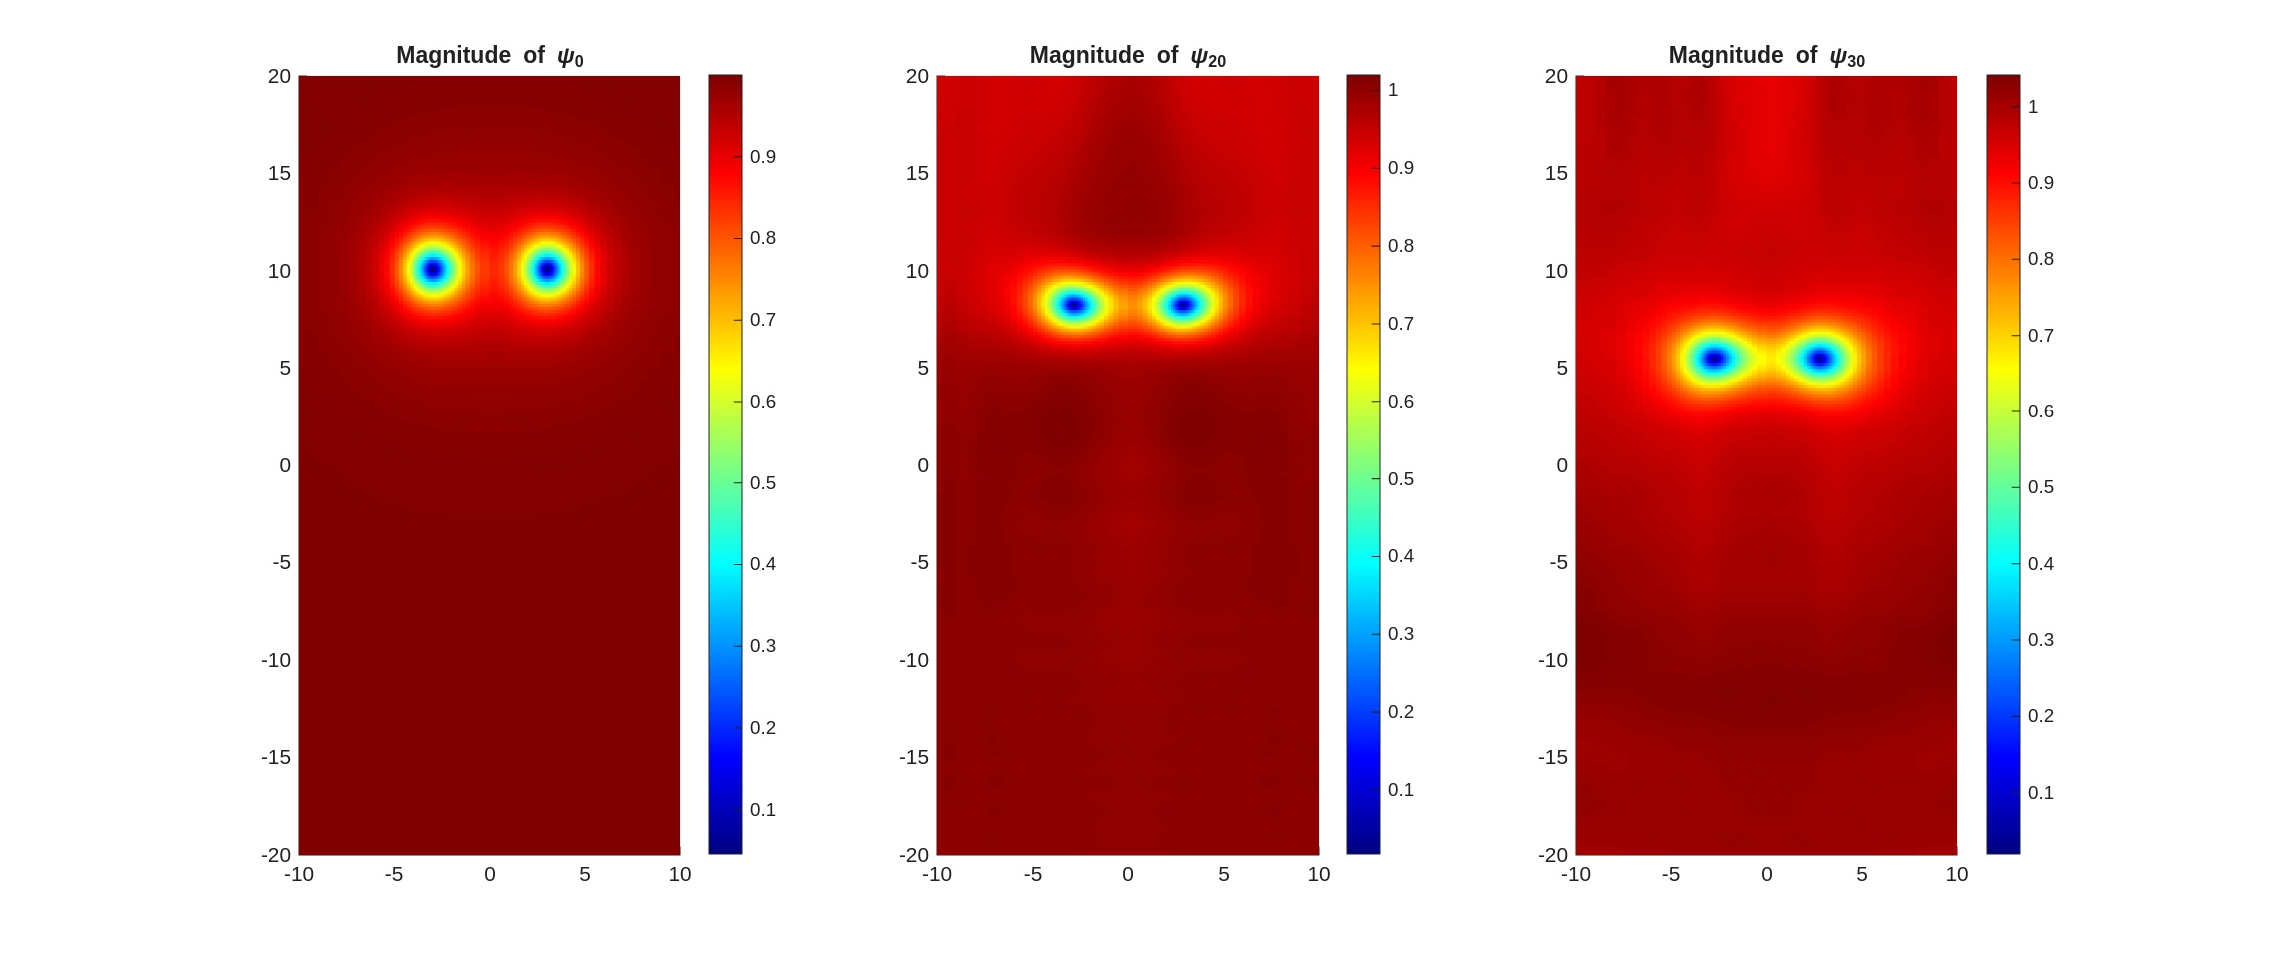
\includegraphics[width=\textwidth]{img/str_01030_3.pdf}
    \caption{Comparison between $\psi_0$ (left), $\psi_{10}$ (center), and $\psi_{30}$ (right), for $x_c = 3$.}
\end{figure}

With this configuration, the vortices appear to ``march'' steadily towards the lateral boundaries of the computational domain. This drift is a direct consequence of the imposed counter-rotation, which breaks the otherwise stationary balance. In the following figure we can appreciate how the translation speed depends strongly on the initial separation between the vortex centers.

\begin{figure}[H]
    \centering
    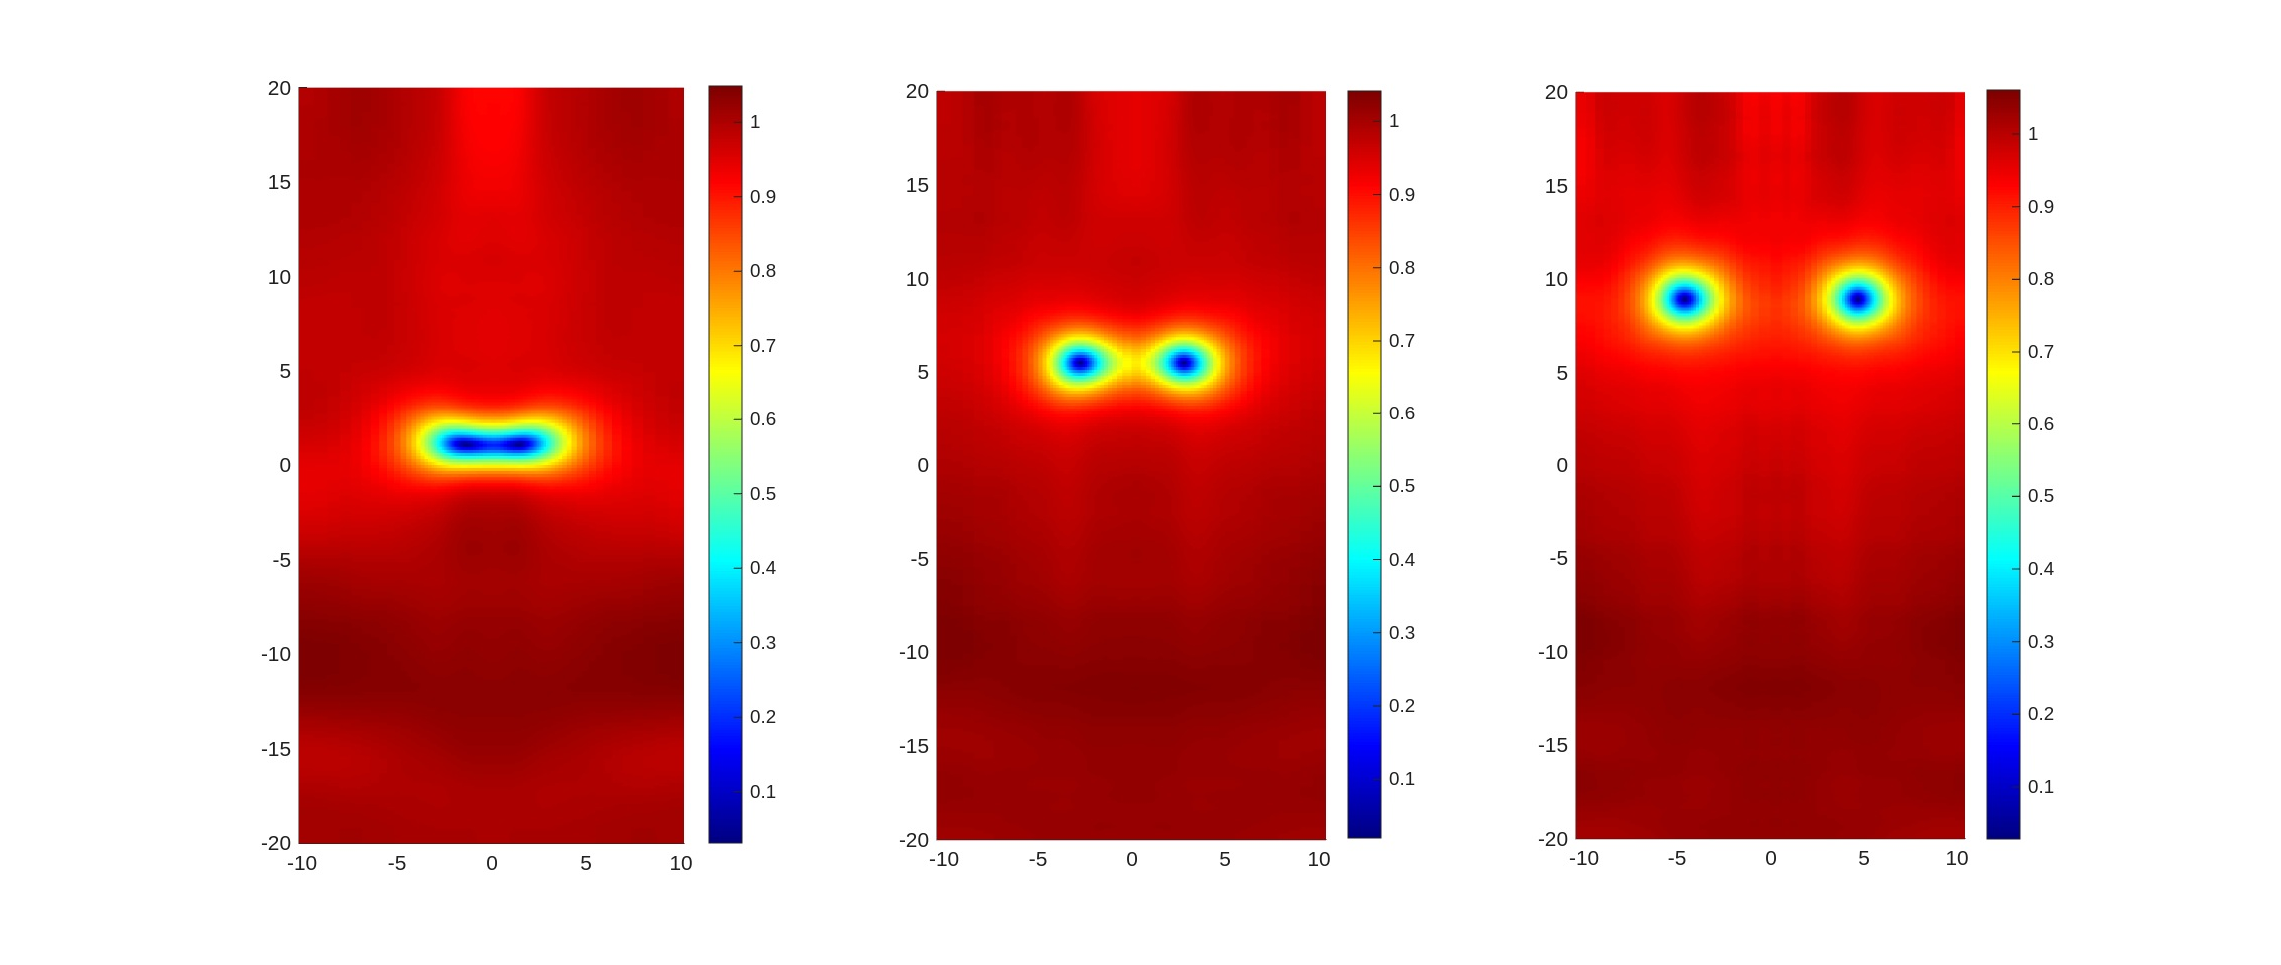
\includegraphics[width=\textwidth]{img/str_235_30t.pdf}
    \caption{Solutions at time $t = 30$ for $x_c = 2, 3,$ and $5$.}
\end{figure}

All simulations reported here were performed on a nonuniform grid along the $x$-direction, with the spacing defined in \ref{sb:nufg}, while in the $y$-direction equispaced nodes were employed. This choice of discretization allows one to concentrate grid resolution where the vortex dynamics are more intense, without excessively increasing the overall computational cost.

\section{Simulation of two rotating vortex}

We now employ the initial condition given by 

\[
    \psi_0 = \sqrt{\rho_1 \rho_2}\exp\left(\ii (S_1 - S_2)\right),
\] 

with $\rho_1 = \rho(x - x_{c_1}, y - y_{c_1})$ and $S_1 = \mathrm{atan2}(y - y_{c_1}, x - x_{c_1})$, while $\rho_2 = \rho(x - x_{c_2}, y - y_{c_2})$ and $S_2 = -\mathrm{atan2}(y - y_{c_2}, x - x_{c_2})$.





\appendix
\chapter{Kroneker products and its properties}

From now on, in this section $I$ denotes the identity matrix.

\begin{definition}
    Let $A \in \mathbb{R}^{m \times n}$ and $B \in \mathbb{R}^{p \times q}$. 
    The \emph{Kronecker product} is defined as
    \[
        A \kron B = 
        \begin{bmatrix}
            a_{11}B & \cdots & a_{1n}B \\
            \vdots & \ddots & \vdots \\
            a_{m1}B & \cdots & a_{mn}B
        \end{bmatrix} \in \mathbb{R}^{mp \times nq}.
    \]
    \label{ch:krondef}
\end{definition}

\begin{example}
\[
    \begin{bmatrix}
        1 & 2 \\
        3 & 4
    \end{bmatrix}
    \kron
    \begin{bmatrix}
        0 & 5 \\
        6 & 7
    \end{bmatrix} 
    =
    \begin{bmatrix}
        0 & 5 & 0 & 10 \\
        6 & 7 & 12 & 14 \\
        0 & 15 & 0 & 20 \\
        18 & 21 & 24 & 28
    \end{bmatrix}.
\]
\end{example}

\begin{proposition}
    If $A,B,C,D$ are matrices of compatible dimensions, then
    \[
        (A \kron B)(C \kron D) = (AC) \kron (BD).
    \]
    \label{prop:prod}
\end{proposition}

\begin{proof}
    The $(i,j)$ block of $(A \kron B)(C \kron D)$ is
    \[
        \sum_k (a_{ik}B)(c_{kj}D) = \Big(\sum_k a_{ik}c_{kj}\Big) BD = (AC)_{ij}BD,
    \]
    which coincides with the $(i,j)$ block of $(AC) \kron (BD)$.
\end{proof}

\begin{proposition}
    Let $A \in \C^{m \times m}$, $B \in \C^{n \times n}$, such that $[A,B] = 0$ and $\uu \in \C^{mn}$. Then 

    \[(A \kron B)\uu = BUA^T\]

    where $\uu = \mathrm{Vec}(U)$, $U_{i,j} =  u_{i + m(j - 1)}$ 

    \label{prop:tensorprod}
\end{proposition}

\begin{proof}
    Considering the product 

    \[
        (A \kron B)\uu = 
        \begin{bmatrix}
            a_{11}B & \cdots & a_{1n}B \\
            \vdots & \ddots & \vdots \\
            a_{m1}B & \cdots & a_{mn}B
        \end{bmatrix}
        \begin{bmatrix}
            u_1 \\
            \vdots \\
            u_{mn}
        \end{bmatrix}
    \]

    we have that the $i$-th component of the resulting vector is 

    \[\sum_{j = 1}^{m}a_{ij}Bu((i - 1)n + 1:in)\]

    where $u(k:\ell)$ denotes the vector $\left[u_k, u_{k+1}, \cdots, u_{\ell}\right]^T$.

    By definition of the matrix $U \in \C^{m \times n}$ such that $\uu = \mathrm{Vec}(U)$, we have

    \[
        u((j-1)n + 1 : j n) = U(j,:) ^T,
    \]

    Given that, we can now rewrite the expression for the $i$-th component of the result.

    \[
        V_{i,:} = \sum_{j = 1}^m a_{i,j} \, B \, U(j,:)^T = \sum_{j = 1}^m (B \, U)_{j,:} \, a_{i,j} 
    \]

\end{proof}

\begin{lemma}
    For every $n \in \mathbb{N}$, one has
    \[
        (I \kron A)^n = I \kron A^n.
    \]
\end{lemma}

\begin{proof}
    By induction on $n$. For $n=1$ the claim is trivial. Suppose it holds for $n-1$; then
    \[
        (I \kron A)^{n} = (I \kron A)(I \kron A)^{n-1} =(I \kron A)(I \kron A^{n-1}) = II \kron AA^{n-1} = I \kron A^{n}
    \]
    where we used the previous proposition.
\end{proof}

\begin{lemma}
    Let $A,B \in \C^{m \times n}$ and $X$ a matrix. Then $X \kron A + X \kron B = X \kron (A + B)$.
\end{lemma}

\begin{proposition}
    Let $\left\{A_k\right\}_{k = 1}^\infty$ be a sequence of matrices, where $A_j \in \C^{m \times n}$ for all $j$. Let $I$ be the identity matrix of arbitrary dimensions. Then 
    \[ \sum_{k = 1}^\infty \left(I_k \kron A_k\right) = I_k \kron \sum_{k = 1}^\infty A_k \]
\end{proposition}

\begin{proof}
    We consider the infinite sum as the limit of a partial sum as $\sum_{k = 1}^\infty \left(I \kron A_k\right) = \lim_{n \to \infty} \sum_{k = 1}^n \left(I \kron A_k\right)$.

    We now proceed for induction on $n$. For $n = 1$ the claim is trivial. Suppose it holds for $n-1$, then 

    \[
        \sum_{k = 1}^n \left(I \kron A_k\right) = I \kron A_n + \sum_{k = 1}^{n-1} \left(I \kron A_k\right) = I \kron A_n + I \kron \sum_{k = 1}^{n-1} A_k = I \kron \sum_{k = 1}^n A_k
    \]
\end{proof}

\begin{theorem}
    Let $f$ be an analytic function. Then
    \[
        f(I \kron A) = I \kron f(A).
    \]
    \label{th:analytic}
\end{theorem}

\begin{proof}
    Write $f(X) = \sum_{k=0}^\infty \alpha_k X^k$. Then
    \[
        f(I \kron A) = \sum_{k=0}^\infty \alpha_k (I \kron A)^k
        = \sum_{k=0}^\infty \alpha_k (I \kron A^k)
        = I \kron \left(\sum_{k=0}^\infty \alpha_k A^k\right)
        = I \kron f(A).
    \]
\end{proof}



\chapter{MATLAB\textsuperscript{\textregistered} implementation}

\bibliographystyle{plain}
\bibliography{reference}

\end{document}